\documentclass{article}
\usepackage{amssymb}
\usepackage[utf8]{inputenc}
\usepackage{graphicx}
\usepackage[a4paper, total={7in, 10in}]{geometry}
\usepackage{subcaption}


\title{Propagation of Deformations in Flocks}
\author{Sacha AMIEL, Léo CONSTANTIN et Théo GLORIEUX}
\date{}

\begin{document}

%https://en.wikipedia.org/wiki/Boids
%http://www.red3d.com/cwr/boids/
%https://eater.net/boids
%https://www.caltech.edu/about/news/engineers-taught-drone-herd-birds-away-airports-82933
%https://www.google.com/url?sa=t&rct=j&q=&esrc=s&source=web&cd=&cad=rja&uact=8&ved=2ahUKEwiCjMPJjJX7AhU0X_EDHTHlAw0QFnoECBkQAQ&url=https%3A%2F%2Fauthors.library.caltech.edu%2F87601%2F2%2Ftro-chung-2853610_final1.pdf&usg=AOvVaw1M0lNJ5fGq5l02ShFUV2ZB
\maketitle

\section*{Context}
The most incredible fact about flocks is that, without any communication on a large scale and without any leadership, individual neighbor-to-neighbor behavior causes the emergence of a global steering capacity; allowing the entire flock to avoid obstacles and stay of a relatively homogeneous density.\\

In 1986, Craig Reynolds created the first flocking simulation \cite{Rey}. To do so, he only used three extremely simple rules named: "alignment - cohesion - separation". The boids (standing for bird-oïd) are the flock's atomic components (like birds of a feather in the sky $3D$, of Galiminii of the same heard in Jurasic Parc $2D$). Each is defined by its position, speed and orientation (hence is a value in $\mathbb{R}^N$).\\
At every step $\mathrm{d}t$ the boïds get updated in the following way:
\begin{itemize}
    \item Alignment: each Boid steers to avoid crowding local flockmates;
    \item Cohesion: steer towards the average heading of local flockmates;
    \item Separation: steer to move towards the average position (center of mass) of local flockmates.
\end{itemize}
\begin{figure}[h]
    \centering
    \begin{subfigure}[b]{0.3\textwidth}
        \centering
        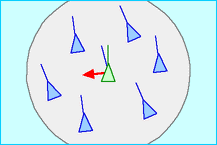
\includegraphics[scale=1.5]{PJ/Images/alignment.png}
        \caption{Alignment}
        \label{fig:alg}
    \end{subfigure}
    \begin{subfigure}[b]{0.3\textwidth}
        \centering
        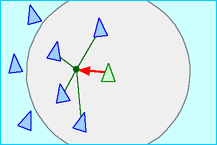
\includegraphics[scale=1.5]{PJ/Images/cohesion.png}
        \caption{Cohesion}
        \label{fig:coh}
    \end{subfigure}
    \begin{subfigure}{0.3\textwidth}
        \centering
        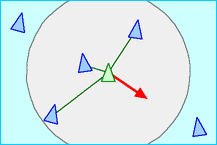
\includegraphics[scale=1.5]{PJ/Images/separation.png}
        \caption{Seperation}
        \label{fig:sep}
    \end{subfigure}
    \caption{Drawings by Craig Reynolds from his webpage \cite{Cra}}
    \label{fig: rules}
\end{figure}


The stinking simplicity of this model is allthemore interesting when one witnesses that is seems to flawlessly recreate real-life flock behaviors, suggesting that those simple rules are the ones followed by real animals. But it also allows for interesting thought experiments such as the following one: if, in flocks, all the individuals just "try to align with there neighbours" if we were to control a single boid in the flock, would this grant us control over the entire flock? This is the question that drove us towards the subject we would like to study:
\begin{center}
\fbox{%
\begin{minipage}{0.98\textwidth}
   We wish to study the propagation of sound (i.e. density variations) in flocks of boids. Both low and high frequencies, both periodic and sudden variations... 
\end{minipage}
}\end{center}\\

The study of this is nothing new, it was already studied in  \cite{Cav} and in \cite{Yuh}. But in both those works, only the "natural noise" arsing from the boids themselves was studied. (Indeed, to make the flocks more "realistic" boids are also given a random oscilation arround the theoretical model, and those can be amplified by the flock.) We whish to use hand-controlled boids (called drones) to generate the perturbations. Although this method was never used in simulations (to our knowledge) it was used in real life to gain control over flocks or heards of animal \cite{Ros}, so it must have some physical relevance. \\
 \newpage

\section*{Approach – Method}
 The project will focus on the simulation of a flock in a box with different possible limits.
 by defining a flock as a set of particles coupled to their neighbours we can study the propagation of information within the flock. The flock dynamic can be described with a simple equation:
 \begin{equation}
     \frac{\mathrm{d}\vec{v}_i}{\mathrm{d}t}=-\frac{\partial H}{\partial \vec{v_i}} + \vec{\eta}_i,
     \label{eq1}
 \end{equation}
 \begin{equation}
     \frac{\mathrm{d}\vec{x}_i}{\mathrm{d}t}=\vec{v}_i,
     \label{eq2}
 \end{equation}
  \begin{equation}
     H=\frac{1}{2} J\sum_{i,j=1}^N \eta_{ij}(\vec{v_i}-\vec{v_j})^{2}  +  \sum_{i}^N V(\vec{v_i}),
     \label{eq3}
 \end{equation}
 $H$ is an effective hamiltonian including the interaction between particles' velocity with strength $J$ and a speed control term. $\eta_{ij}$ is 1 for interacting neighbour, 0 otherwise.
 discretizing \ref{eq1} and \ref{eq2}, we can use an Euler integration to solve our problem.
 
 
 We can also model our flocks, in the continuum limit, by replacing our boids by two fields: the density field of boids $\rho(\vec{x},t)$ and the velocity field $\vec{v}(\vec{x},t)$. Those fields verify:
 \begin{equation}
     \frac{\partial \vec{v}}{\partial t} + \lambda(\vec{v}.\vec{\nabla})\vec{v} = \alpha \vec{v} - \beta||\vec{v}||^2\vec{v} -\vec{\nabla}P +D_L \vec{\nabla} (\vec{\nabla}. \vec{v}) + D_1\Delta\vec{v}+ D_2(\vec{v}.\vec{\nabla})^2\vec{v} +\vec{f}
 \end{equation}
 
 \begin{equation}
     \frac{\partial\rho}{\partial t} + \vec{\nabla}.(\rho\vec{v})=0
 \end{equation}
 
 Where $D_L, D_1, D_2$ and $\beta \in\mathbb{R}^*_+$. $D_L,D_1$ and $D_2$ are diffusion constants, $\beta\in\mathbb{R}^*_+, \alpha\in\mathbb{R}$. The sign of $\alpha$ gives us the state of the system ($\alpha > 0$: ordered state, $\alpha<0$: unordered state). $\vec{f}$ represents the Gaussian random noise. It has the correlations $<f_i(\vec{r},t)f_j(\vec{r'},t')>= A\delta_{ij} \delta^d(\vec{r}-\vec{r'})\delta(t-t')$ where $i,j\in[|0;d|]$ and $A\in\mathbb{R}$. The pressure P is defined by $P=P(\rho)=\sum_{n=0}^{+\infty} \sigma_n(\rho-\rho_0)^n$ where $\rho_0$ is the mean value of the density of boids and the $\sigma_n$ are the coefficients.
 
 We will resolve those equations using numerical methods and we will compare those results with the ones we will obtain with numerical methods. 

\section*{Observations and expected results:}
    We would like to:
    \begin{enumerate}
        \item visualize our flock
        \item plot the evolution of the density of the flock (can a perturbation cause boids to "crash" into one another?)
        \item plot the speed distribution
    \end{enumerate}
Here some other interesting things we may take a look at:
\begin{itemize}
    \item The influence of the number of drones and there distribution;
    \item The influence of the shape of the perturbation (planar, circular... periodic or not...);
    \item The evolution of the shape of the flock (can a perturbation make a flock more or less spherical, or can it separate the flock, or how will it separate the flock).
\end{itemize}

\bibliographystyle{unsrt}
\bibliography{PJ/Biblio.bib}
\end{document}
